\chapter{Advice for Applying Machine Learning}

\section{Evaluating a Hypothesis}

Once we have done some trouble shooting for errors in our predictions by:
\begin{itemize}
\item Getting more training examples
\item Trying smaller sets of features
\item Trying additional features
\item Trying polynomial features
\item Increasing or decreasing $\lambda$
\end{itemize}

We can move on to evaluate our new hypothesis.\\

A hypothesis may have a low error for the training examples but still be inaccurate (because of overfitting). Thus, to evaluate a hypothesis, given a dataset of training examples, we can split up the data into two sets: a training set and a test set. Typically, the training set consists of 70 \% of your data and the test set is the remaining 30 \%.\\

The new procedure using these two sets is then:\\

\begin{enumerate}
\item Learn $\Theta$ and minimize $J_{train}(\Theta)$ using the training set.
\item Compute the test set error $J_{test}(\Theta)$
\end{enumerate}

\subsection{The test set error}

\begin{enumerate}
\item For linear regression: $$J_{test} (\Theta) =\frac{1}{2m_{test}}\sum_{i=1}^{m_{test}}(h_\Theta(x^{(i)}_{test})-y^{(i)}_{test})^2 $$

\item For classification $\rightarrow$ Misclassification error (aka 0/1 misclassification error):

\begin{center}
$err(h_\Theta(x),y) = \begin{cases} 1, & \mbox{if } h_\Theta(x) \geq 0.5  \mbox{ and } y=0 \mbox{ or } h_\Theta(x) < 0.5 \mbox{ and } y=1 \\ 0, & \mbox{otherwise } \end{cases}$
\end{center}
\end{enumerate}

This gives us a binary 0 or 1 error result based on a misclassification. The average test error for the test set is:

\begin{center}
$$\mbox{Test Error = } \frac{1}{m_{test}}\sum_{i=1}^{m_{test}}err(h_\Theta(x^{(i)}_{test})-y^{(i)}_{test})$$
\end{center}

This gives us the proportion of the test data that was misclassified.


\section{Model Selection and Train/Validation/Test Sets}

Just because a learning algorithm fits a training set well, that does not mean it is a good hypothesis. It could over fit and as a result your predictions on the test set would be poor. The error of your hypothesis as measured on the data set with which you trained the parameters will be lower than the error on any other data set.\\

Given many models with different polynomial degrees, we can use a systematic approach to identify the 'best' function. In order to choose the model of your hypothesis, you can test each degree of polynomial and look at the error result.\\

One way to break down our dataset into the three sets is:

\begin{itemize}
\item Training set: 60\%
\item Cross validation set: 20\%
\item Test set: 20\%
\end{itemize}

We can now calculate three separate error values for the three different sets using the following method:

\begin{enumerate}
\item Optimize the parameters in $\Theta$ using the training set for each polynomial degree.
\item Find the polynomial degree \textit{d} with the least error using the cross validation set.
\item Estimate the generalization error using the test set with $ J_{test}(\Theta^{(d)}) $, (\textit{d }= theta from polynomial with lower error);
\end{enumerate}

This way, the degree of the polynomial \textit{d} has not been trained using the test set.

\section{Diagnosing Bias vs. Variance}

In this section we examine the relationship between the degree of the polynomial \textit{d} and the underfitting or overfitting of our hypothesis.\\

We need to distinguish whether bias or variance is the problem contributing to bad predictions, given that \textbf{high bias is underfitting} and \textbf{high variance is overfitting}. Ideally, we need to find a golden mean between these two.\\

The training error will tend to decrease as we increase the degree \textit{d} of the polynomial. At the same time, the cross validation error will tend to decrease as we increase \textit{d} up to a point, and then it will increase as \textit{d} is increased, forming a convex curve.\\

\begin{tcolorbox}[width=\textwidth,colback={white},colbacktitle=white]
\textbf{High bias (underfitting)}: both $ J_{train}(\Theta) $ and $ J_{CV}(\Theta) $ will be high. Also, $ J_{CV}(\Theta) \approx J_{train}(\Theta) $.\\

\textbf{High variance (overfitting)}: $ J_{train}(\Theta) $ will be low and $ J_{CV}(\Theta)$ will be much greater than $ J_{train}(\Theta) $.
\end{tcolorbox}

The is summarized in the figure below:\\

\begin{figure}[h!]
	\centering
	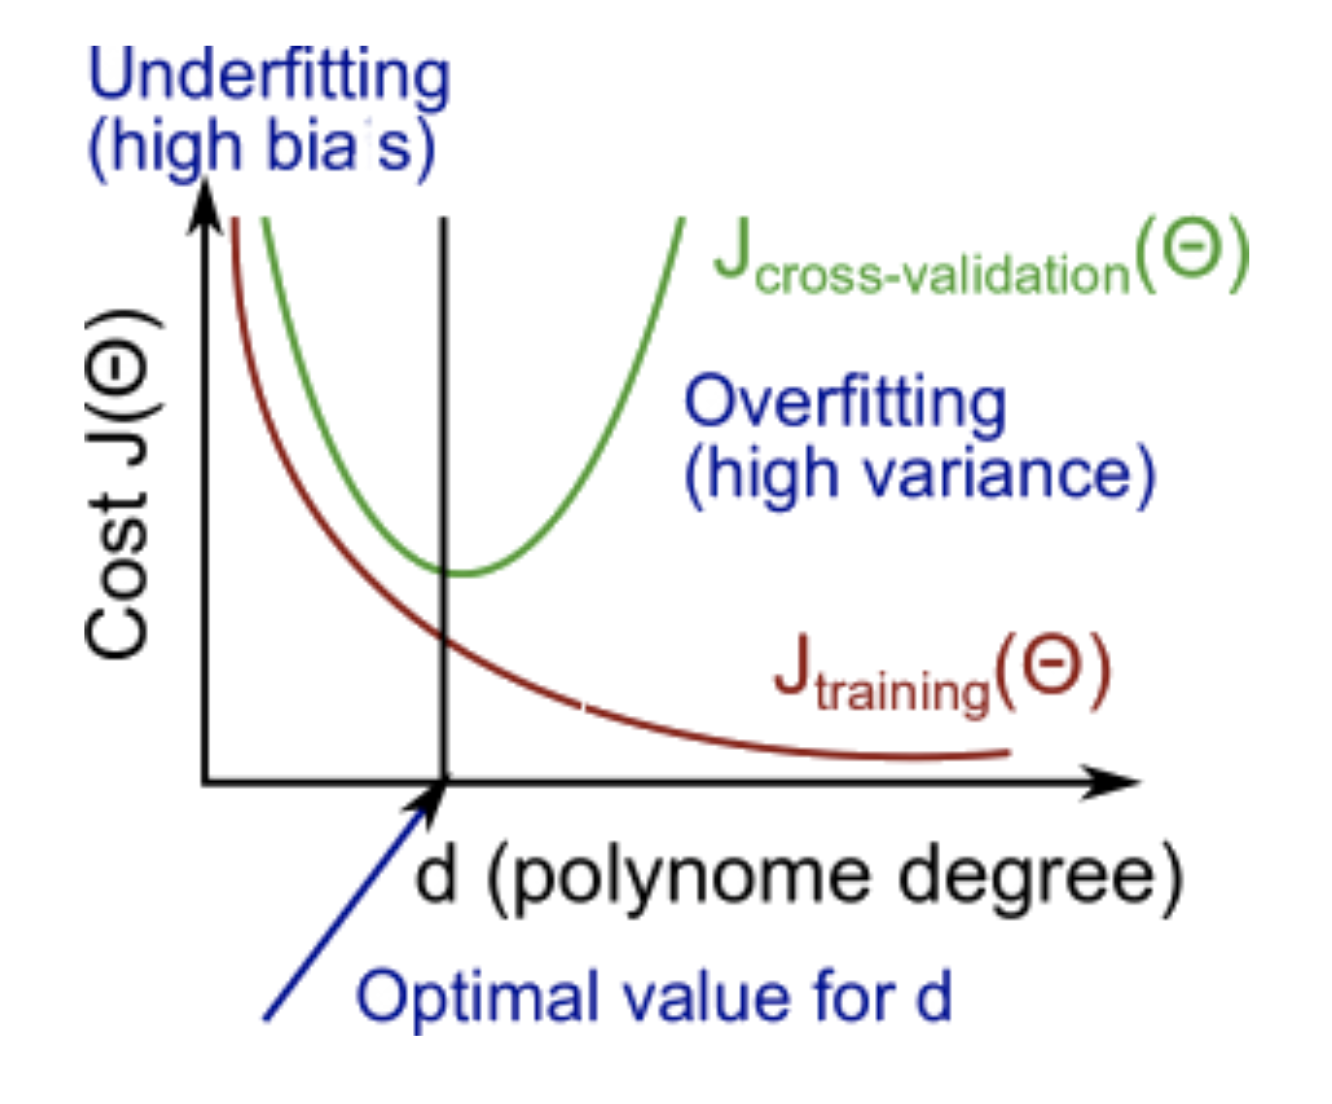
\includegraphics[width=0.5\textwidth]{fig/hv_hb}
	\caption{Optimal value for the degree \textit{d} of the polynomial}
\end{figure}

\section{Regularization and Bias/Variance}

We can see that as $ \lambda $ increases, our fit becomes more rigid. On the other hand, as $ \lambda $ approaches 0, we tend to overfit the data. So how do we choose our parameter $ \lambda $ to get it 'just right' ? In order to choose the model and the regularization term $ \lambda $, we need to:\\

\begin{enumerate}
\item Create a list of lambdas (i.e. $ \lambda \int $ \{0,0.01,0.02,0.04,0.08,0.16,0.32,0.64,1.28,2.56,5.12,10.24\});
\item Create a set of models with different degrees or any other variants.
\item Iterate through the $ \lambda $ and for each $ \lambda $ go through all the models to learn some $\Theta$.
\item Compute the cross validation error using the learned $\Theta$ (computed with $\lambda$) on the $J_{CV}(\Theta)$ without regularization or $ \lambda = 0$.
\item Select the best combo that produces the lowest error on the cross validation set.
\item Using the best combo $\Theta$ and $ \lambda $, apply it on $J_{test}(\Theta)$ to see if it has a good generalization of the problem.
\end{enumerate}


\section{Learning Curves}

Training an algorithm on a very few number of data points (such as 1, 2 or 3) will easily have 0 errors because we can always find a quadratic curve that touches exactly those number of points. Hence:

\begin{itemize}
\item As the training set gets larger, the error for a quadratic function increases.
\item The error value will plateau out after a certain m, or training set size.
\end{itemize}

\textbf{Experiencing high bias:}\\

\begin{tcolorbox}[width=\textwidth,colback={white},colbacktitle=white]
\textbf{Low training set size}: causes $ J_{train}(\Theta) $  to be low and $ J_{CV}(\Theta) $  to be high.\\

Large training set size: causes both $ J_{train}(\Theta) $  and $ J_{CV}(\Theta) $  to be high with $ J_{train}(\Theta) \approx  J_{CV}(\Theta) $ .
\end{tcolorbox}

If a learning algorithm is suffering from \textbf{high bias}, getting more training data will not (\textbf{by itself}) help much.\\

\begin{figure}[h!]
	\centering
	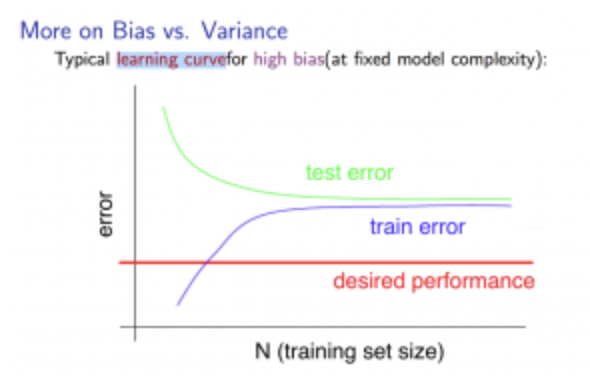
\includegraphics[width=0.6\textwidth]{fig/bias}
	\caption{High Bias}
\end{figure}

\pagebreak

\textbf{Experiencing high variance}:\\

\begin{tcolorbox}[width=\textwidth,colback={white},colbacktitle=white]
\textbf{Low training set size}: $ J_{train}(\Theta) $  will be low and $ J_{CV}(\Theta) $  to be high.\\

Large training set size: $ J_{train}(\Theta) $  increases with training set size and $ J_{CV}(\Theta) $  continues to decrease without leveling off. Also, $ J_{train}(\Theta) <  J_{CV}(\Theta) $ but the difference between them remains significant. .
\end{tcolorbox}

If a learning algorithm is suffering from \textbf{high variance}, getting more training data is \textbf{likely} to help.

\begin{figure}[h!]
	\centering
	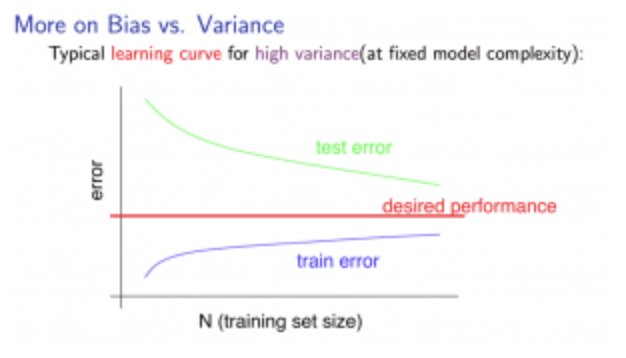
\includegraphics[width=0.6\textwidth]{fig/variance}
	\caption{High Variance}
\end{figure}

\pagebreak

\section{Deciding What to Do Next}

\begin{table}[h!]
	\caption{Decision process}
	\centering
	\begin{tabular}{|l|l|}
		\hline
		\multicolumn{1}{|c|}{\textbf{Fixes High BIAS}} & \multicolumn{1}{c|}{\textbf{Fixes High VARIANCE}} \\ \hline
		Adding features                                & Getting more training examples                    \\
		Adding polynomial features                     & Trying smaller sets of features                   \\
		Decreasing $\lambda$                           & Increasing $\lambda$                              \\ \hline
	\end{tabular}
\end{table}

\subsection{Diagnosing Neural Networks}

\begin{itemize}
\item A neural network with fewer parameters is prone to underfitting. It is also computationally cheaper.
\item A large neural network with more parameters is prone to overfitting. It is also computationally expensive. In this case you can use regularization (increase $\lambda$) to address the overfitting.
\end{itemize}

Using a single hidden layer is a good starting default. You can train your neural network on a number of hidden layers using your cross validation set. You can then select the one that performs best.

\subsection{Model Complexity Effects}

\begin{itemize}
\item Lower-order polynomials (low model complexity) have high bias and low variance. In this case, the model fits poorly consistently.
\item Higher-order polynomials (high model complexity) fit the training data extremely well and the test data extremely poorly. These have low bias on the training data, but very high variance.
\item In reality, we would want to choose a model somewhere in between, that can generalize well but also fits the data reasonably well.
\end{itemize}